%\documentclass[a4paper,english,11pt,twoside]{article}
\documentclass[a4paper,english,11pt]{article}

\usepackage[utf8]{inputenc}
\usepackage[T1]{fontenc, url}
\usepackage[english]{babel}
%\usepackage{epsfig}
\usepackage{graphicx}
\usepackage{amsmath}
\usepackage{mathtools}
\usepackage{pstricks}
\usepackage{subfig}
\usepackage{epstopdf}
\usepackage{varioref}
\usepackage{listings}
\usepackage{xcolor}
\usepackage{float}
\usepackage[]{mcode}
\usepackage{verbatim}
\lstset{ 
  captionpos=b,
  frame=tb,
  numbers=left}
\urlstyle{sf}
\usepackage[margin=1 in]{geometry} % Setter margene til word standard

\usepackage{ifikompendiumforside}


\newcommand{\tab}[1]{\hspace{.2\textwidth}\rlap{#1}}

\newcommand{\itab}[1]{\hspace{0em}\rlap{#1}}

%%%%%%%%%%%%%%%%%% END HEADER

\title{Laboratory Assignment 2}
\subtitle{INF4411\\ 
          Analog Microelectronics}

\author{
\begin{tabular}{ r c l }
  Rikesh Chauhan & & rikesh.chauhan@fys.uio.no\\
  Espen Klein Nilsen & & e.a.k.nilsen@fys.uio.no\\
  Vegard Midtbøen & & vegard.midtboen@fys.uio.no
\end{tabular}
}
%{Rikesh Chauhan rikesh.chauhan@fys.uio.no\\
%	Espen Klein Nilsen e.a.k.nilsen@fys.uio.no\\
%	Vegard Midtbøen vegard.midtboen@fys.uio.no} 

\begin{document}
\ififorside
%//////////////////////////////////////Task1///////////////////////////////////////////////////////////////////////        
\section{Task 1}
The first task was to find a proper bias voltage in order to get a pMOS transitor to deliver a current of $20 \mu A$.
We chose Vdd to be $5 V$, which is enough for this task (Vds = 5V). This voltage is fixed trough the whole experiment.\\
\\
The circut is shown in Figure \ref{fig:sch:task1}. In order to get a proper bias voltage ($V_{p_bias1}$), 
we used a potentiometer of $10k\Omega$. This voltage was found to be $1.96 V$ in order to mach the given drain current.\\
\\
\begin{figure}[htbp]
 \centering
  \fbox{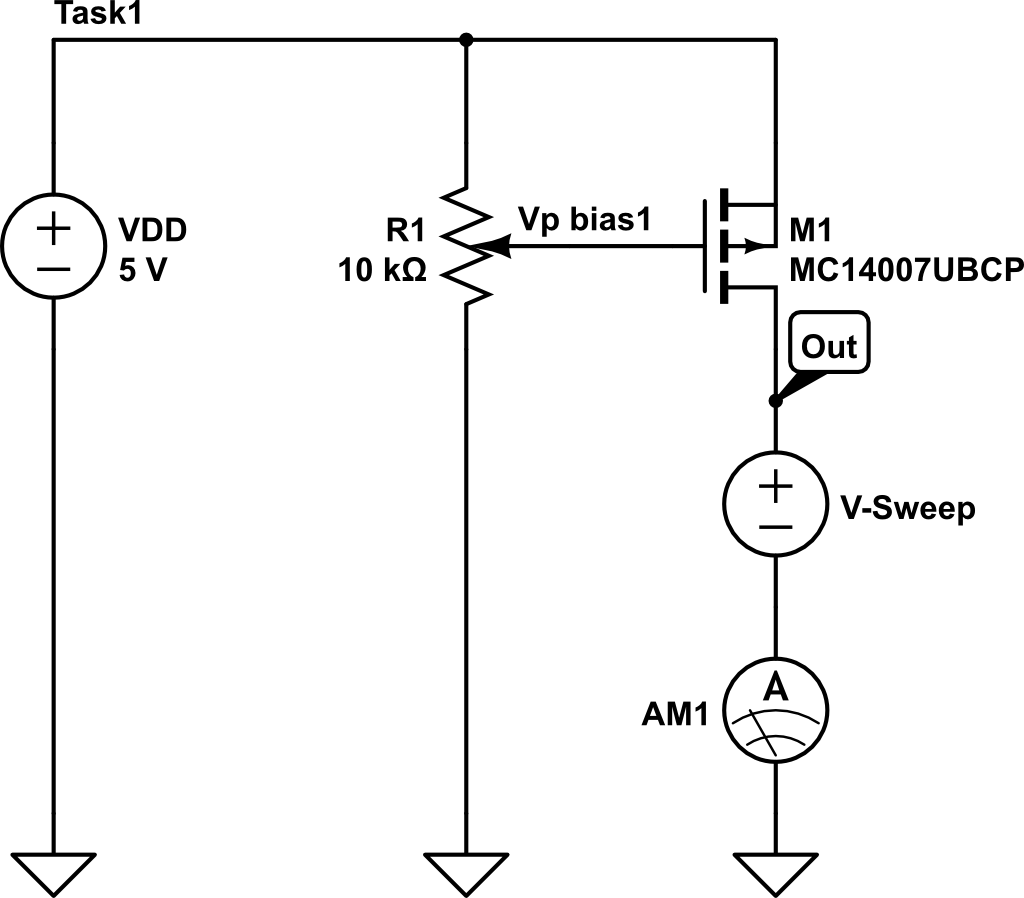
\includegraphics[width=0.5\textwidth]{img/inf4411_lab2_task1_schematics.png}}
  \caption{Transistor setup.}
  \label{fig:sch:task1}	
\end{figure}
The result of the experiment is shown in the Figure \ref{fig:pmos-as-current-source}.\\
\\
\begin{figure}[htbp]
 \centering
  \fbox{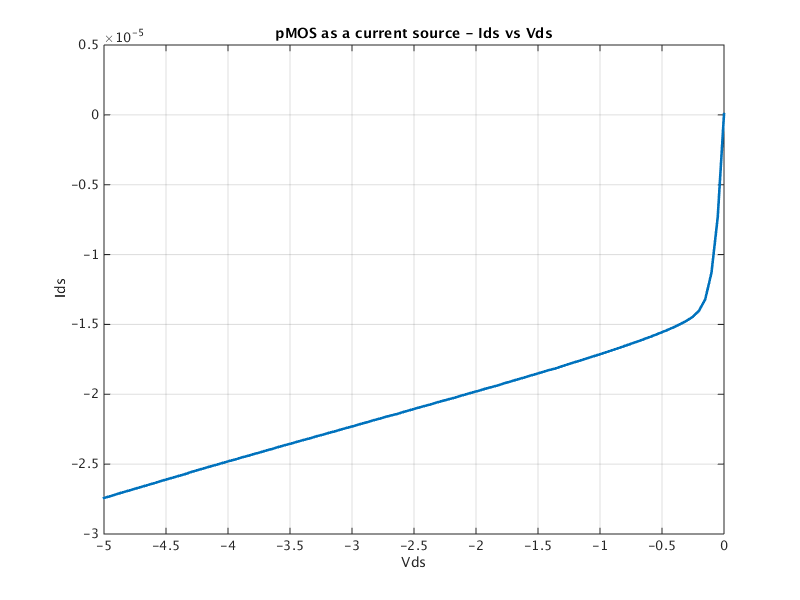
\includegraphics[width=\textwidth]{img/task1_pmos_as_a_current_source.png}}
  \caption{pmos as a current source.}
  \label{fig:pmos-as-current-source}	
\end{figure}
The minimal Vout for this cuircuit to act as an current source is $Vdd - Vds = Vout$, $5 V - 0.5 V = 4.5 V$
Since we probably want to be able to have an AC input, we need some headroom in order to acomodate the signal, both in the positive and negative direction from the setpoint.
The amount of headroom should be big enugh so the transistor never goes out of the active region.*********

\colorbox{red!30}{FIXME}\\
When we selected the V$_{p_bias1}$, we coupled up the circuit as shown in figure (figure ref). In the labdescription it was
gived that the bias current should be 20$\mu$A for the transistor to be in the active region.
V$_{p\_bias}$ = 1.196V\\
rds = 391k$\varOmega$\\
minimal V$_{out}$ = 1.818V\\
Headroom voltage is required to keep the device in active region MORE DETAILS!\\
\colorbox{red!30}{ENDFIXME}\\
    



\begin{figure}[htbp]
 \centering
  \fbox{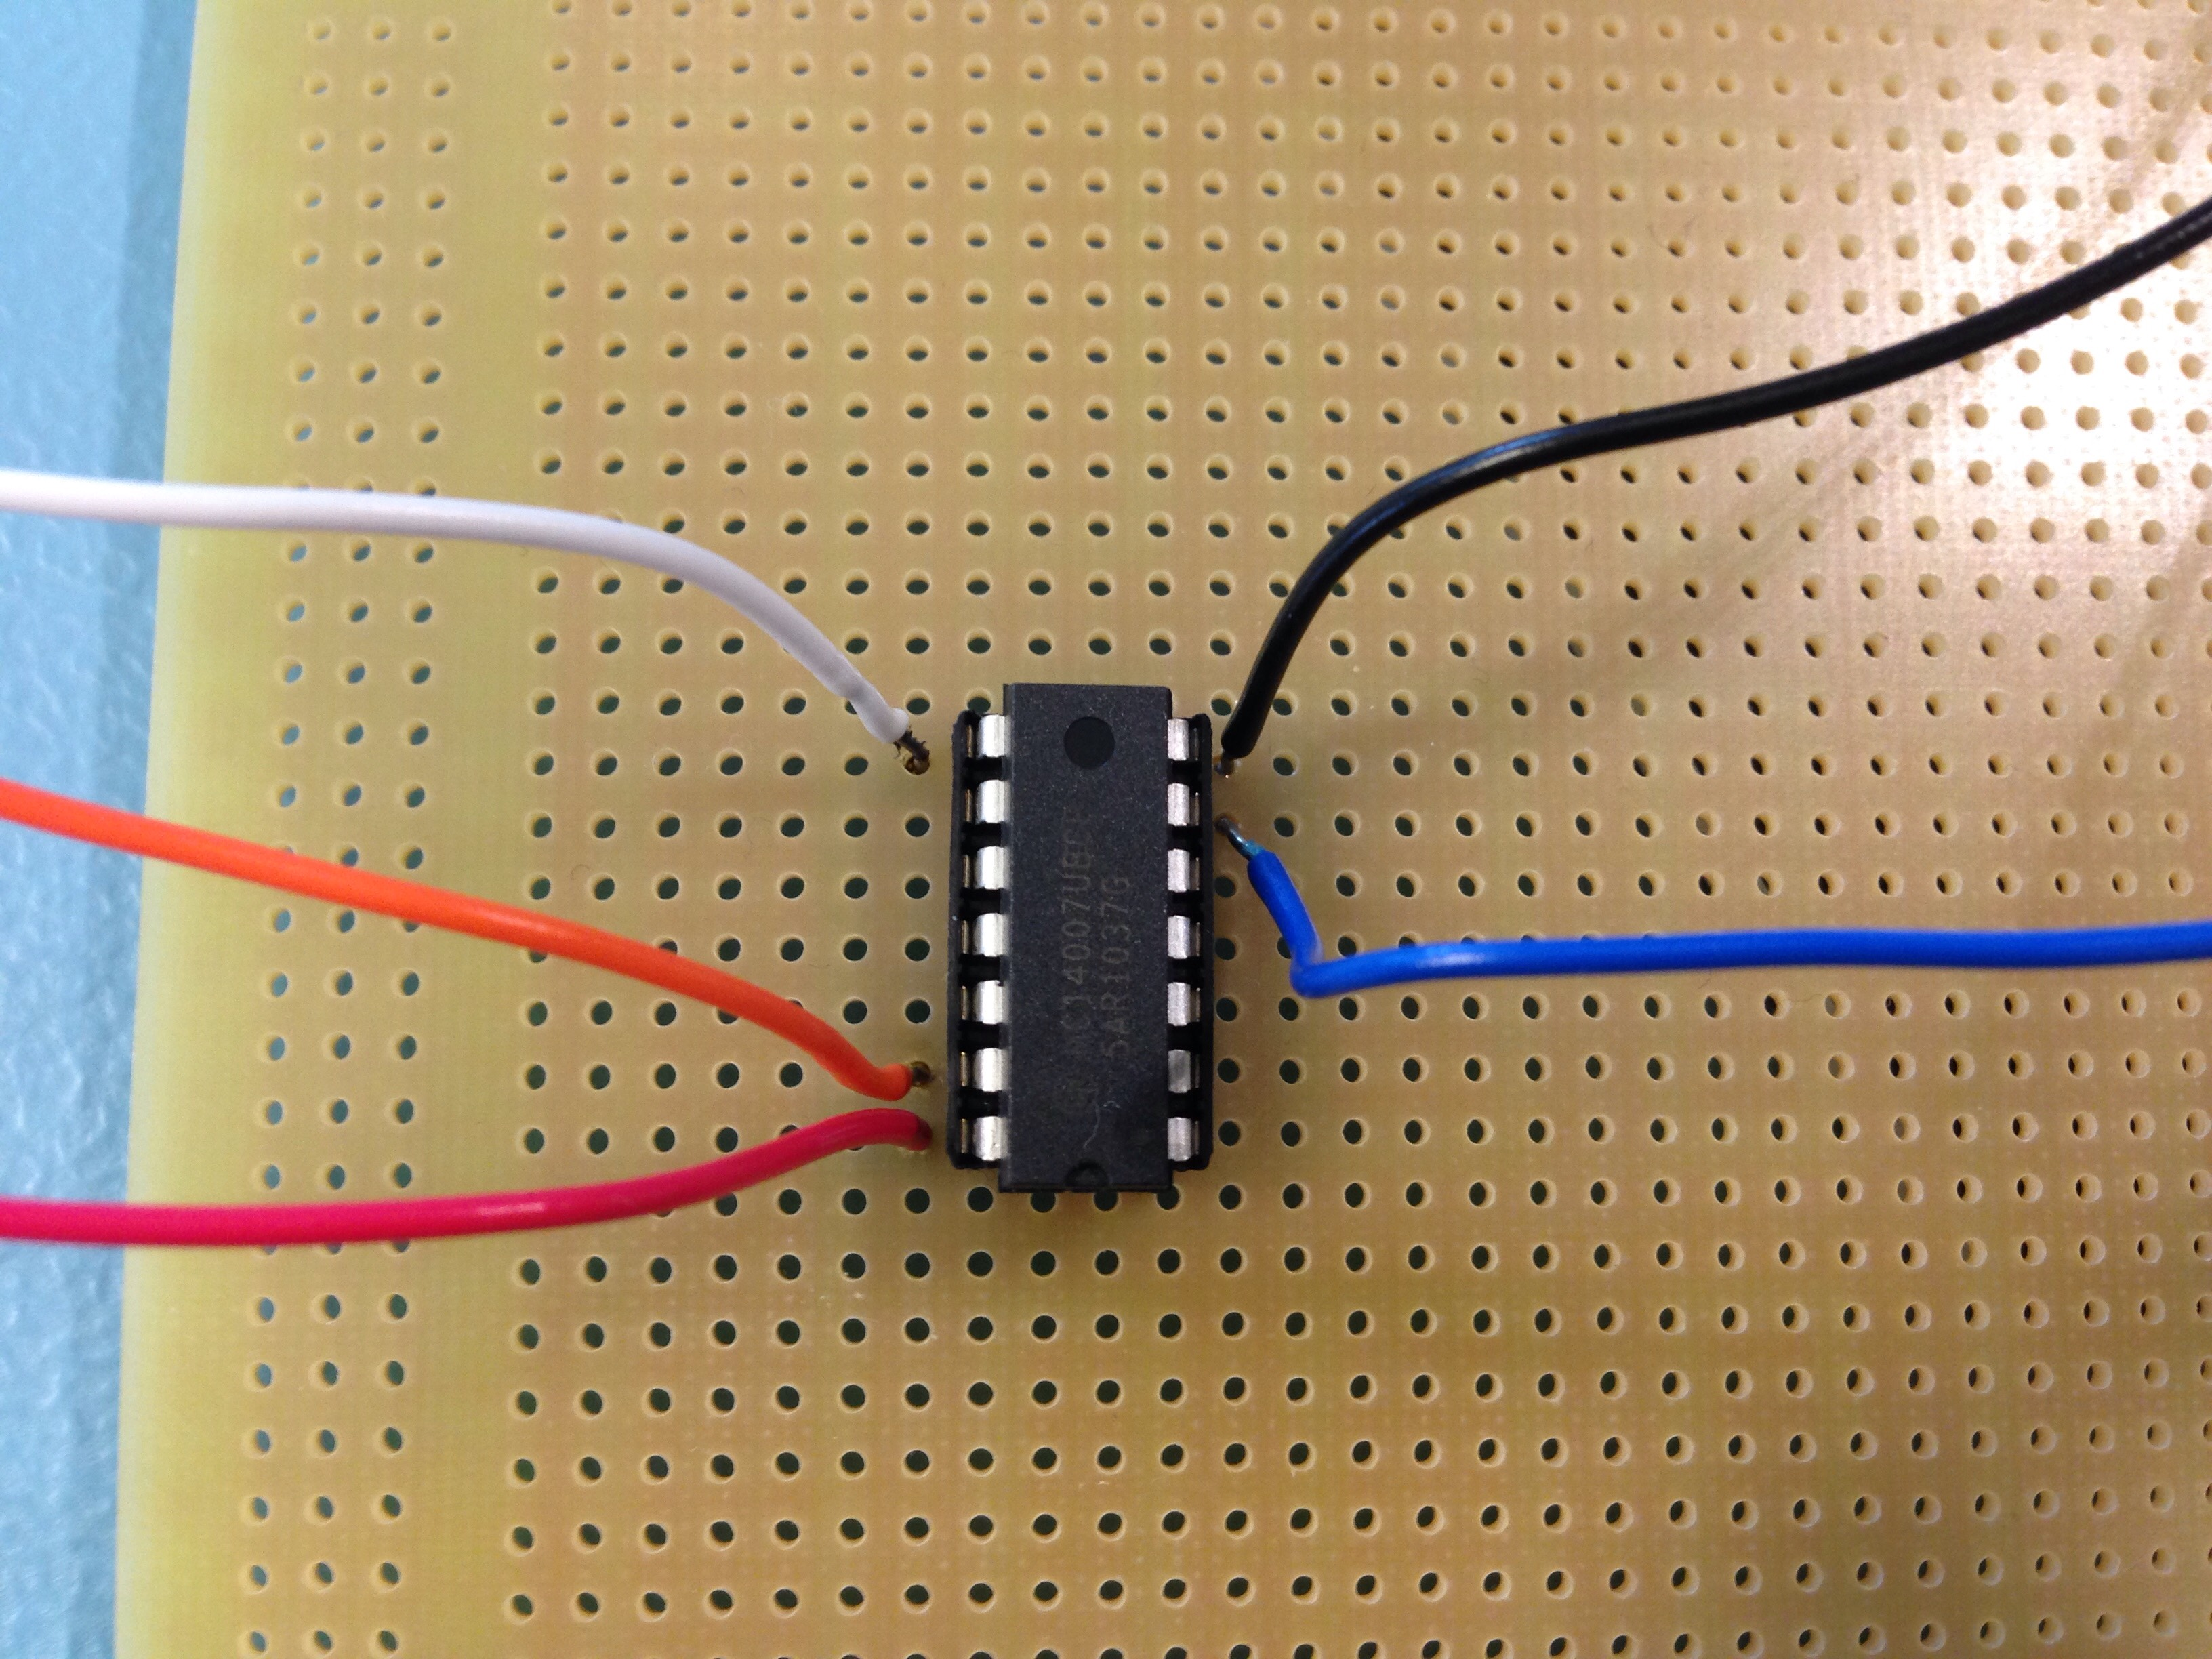
\includegraphics[width=\textwidth]{img/Transistor_setup.jpg}}
  \caption{Transistor setup.}
  \label{fig:tran-setup}	
\end{figure}



\newpage
%//////////////////////////////////////Task2///////////////////////////////////////////////////////////////////////
\section{Task 2}
Now we extend our circut to a current source with a cascode transistor. This is transistor also need proper biasing. The bias for new transistor is also set by potensiometer as seen i figure *****REF.
Now the minimal voltage difference between Vdd and V$_{p_bias2}$ is ************ in order to get the cuircuit to act as an constant current source.
Figure ***** shows a plot of the \colorbox{blue!30}{output current} as a function of V$_{out}$. \\
The output resistance of this cuircuit is estmated to ***********.\\
The minimial voltage $Vdd - V_{out}$ for the cuircuit is ***************.\\


\colorbox{red!30}{FIXME}\\
Notes:\\
- Used two potentiometers to make the desirable voltage for V$_{p_bias1}$ and V$_{p_bias2}$.\\
- VDD (+25V port) = 5V\\
- V$_{sweep}$ = 2.5V\\
- V$_{p_bias1}$ = 1.196V (From last task)\\
- V$_{p_bias2}$ = 3.39V at 20 $\mu$ A\\
- Minimum voltage different is VDD - V$_{p\_bias2}$ = 5V - 3.39V = \underline{\underline{1.61V}}\\
- Minimun output voltage is 2.83V as seen in Figure \ref{fig:pfet-cascode-pfet}.\\
- Output resistance is 13.35M$\Omega$\\
\\
\colorbox{red!30}{ENDFIXME}\\

Figure \ref{fig:pfet-cascode-pfet} shows plot of output current as function of V$_{out}$.
\begin{figure}[htbp]
 \centering
  \fbox{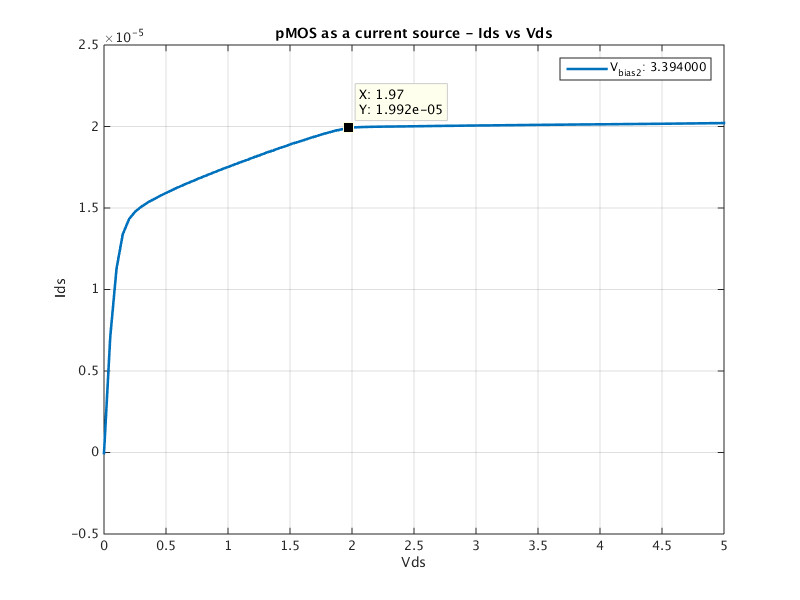
\includegraphics[width=\textwidth]{img/task2_pmos_as_a_current_source.png}}
  \caption{pFET and cascode pFET as a current cource.}
  \label{fig:pfet-cascode-pfet}	
\end{figure}

%//////////////////////////////////////Task3///////////////////////////////////////////////////////////////////////
\section{Task 3}
Using the results form task 1 and task 2 we can estimate values for $V_{eff}$ and the treshold voltage $V_{tp}$.
For task 1 $V_{eff}$ is calculated from the relationship $Vdd - V_{out}$. For task 2 $V_{eff}$ is calculated from the relationship between $V_{out}$ and $V_{p_bias2}$
\\
In task 1 we found the minimal voltage for $Vdd - V_{out}$ to be **************. Using this value to estimate $V_{eff}$ we get ***********.\\
\\
Our results are consistent/not-consistent.....

\newpage
%//////////////////////////////////////Task4///////////////////////////////////////////////////////////////////////
\section{Task 4}
In this task we were supose to use two nMOS transistors and repete what we did in task 2. Figure \ref{fig:sch:task4} shows the shematics for this setup. 
Since the package that was used for the previous task only can be configured for three different gate voltages, we had to add an extra package.\\
\begin{figure}[htbp]
 \centering
  \fbox{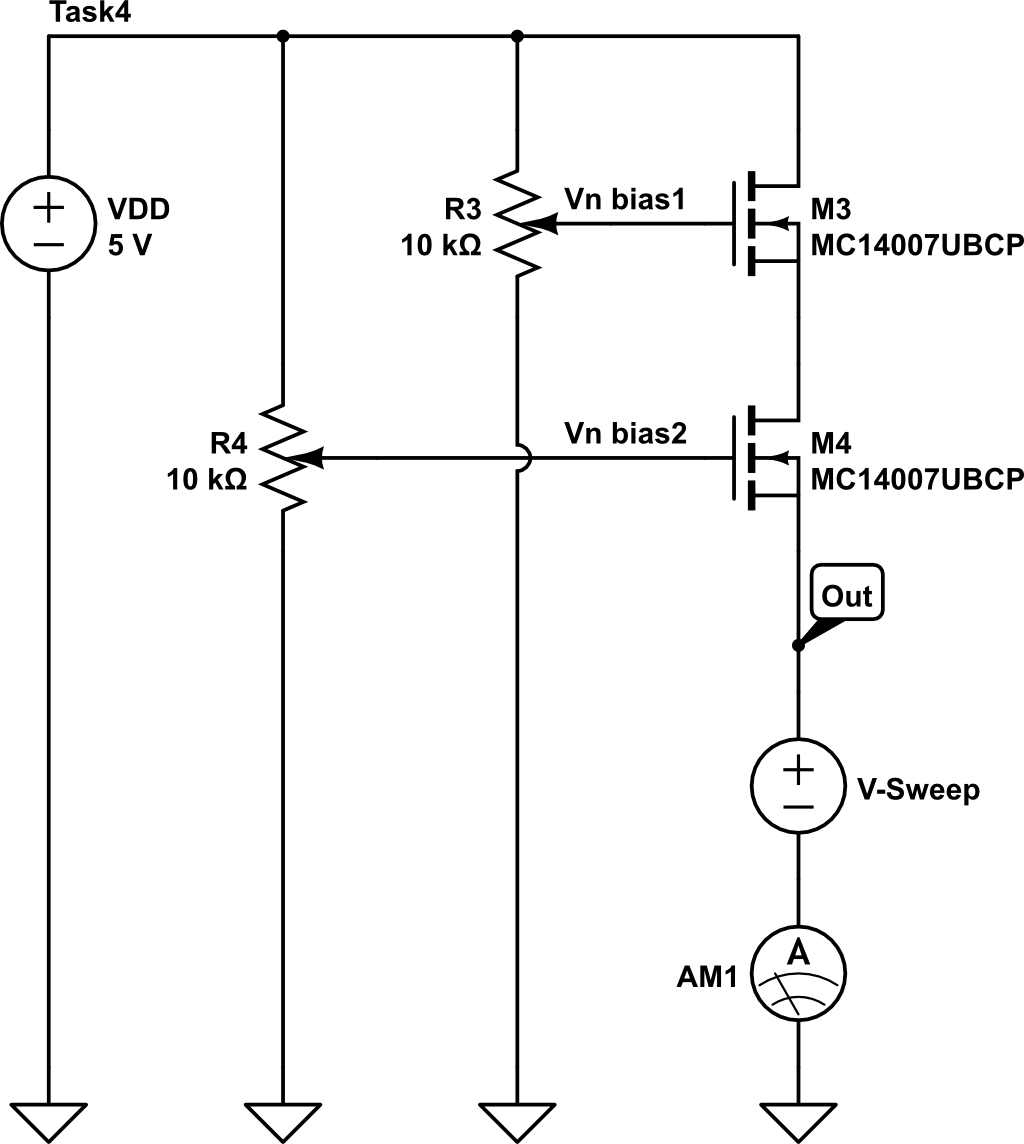
\includegraphics[width=0.5\textwidth]{img/inf4411_lab2_task4_schematics}}
  \caption{nMOS transistor setup.}
  \label{fig:sch:task4}	
\end{figure}
\begin{figure}[htbp]
 \centering
  \fbox{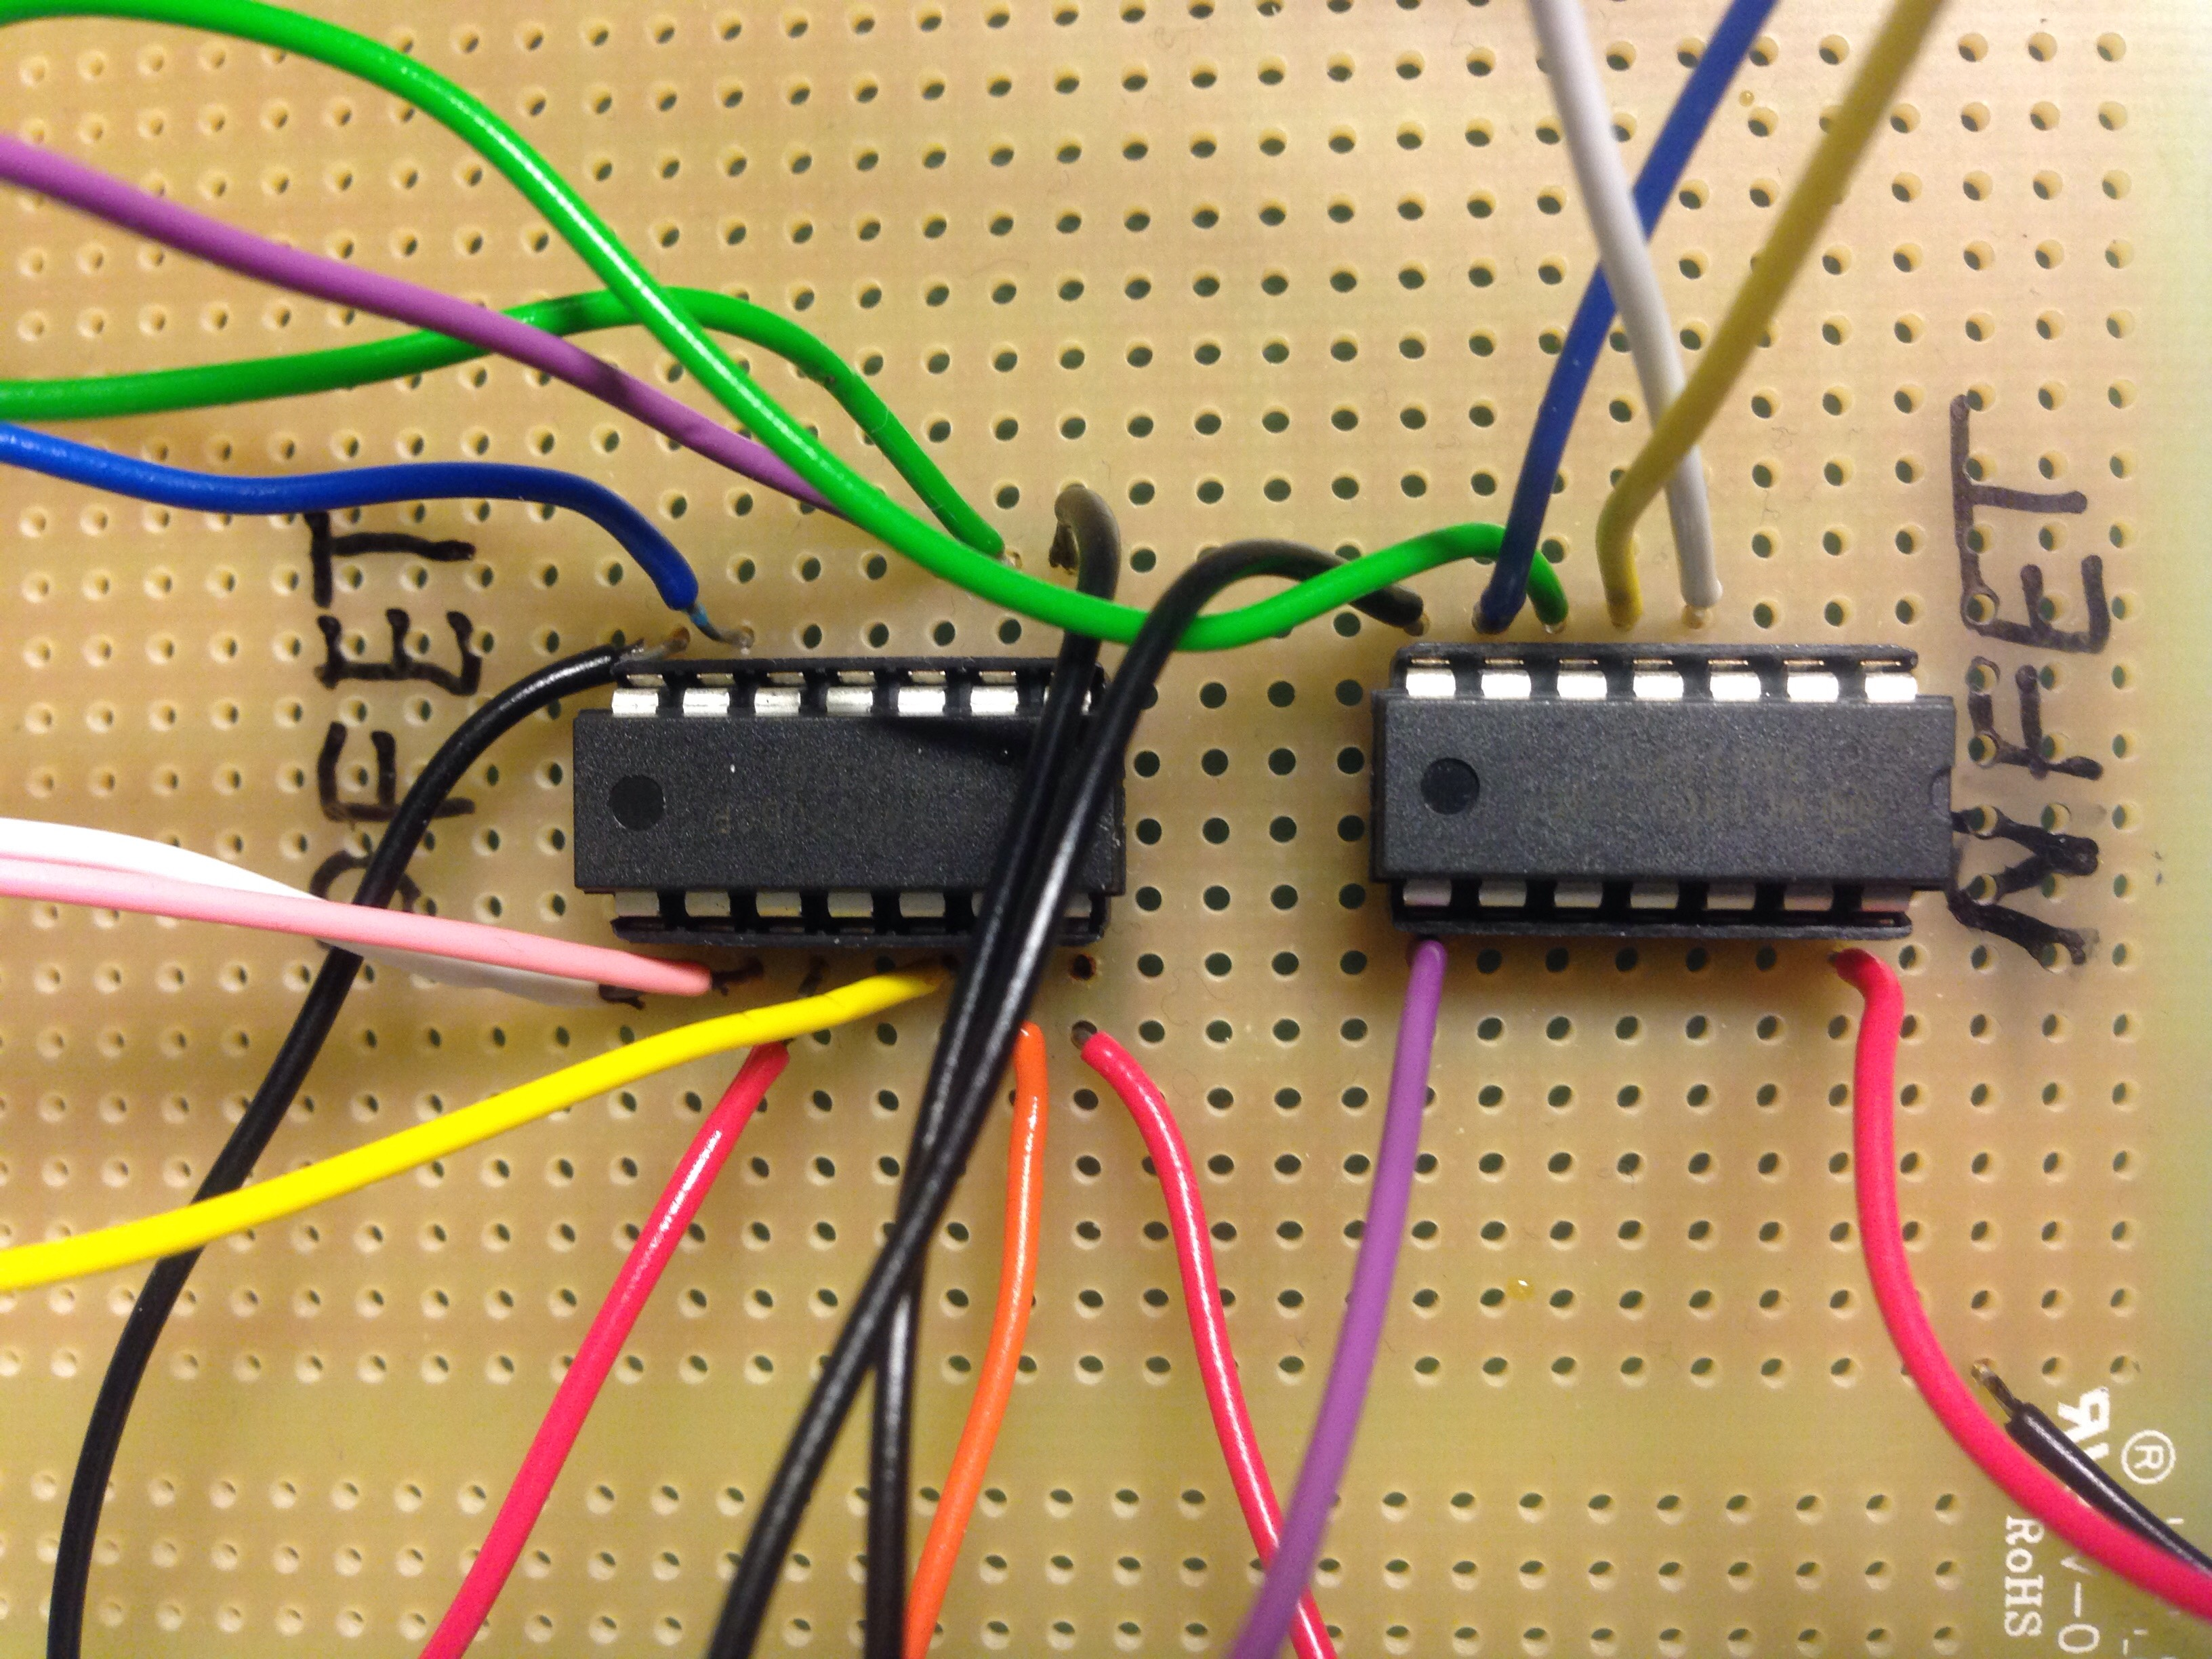
\includegraphics[width=0.6\textwidth]{img/pmos_and_nmos_setup}}
  \caption{pMOS and nMOS PCB setup.}
  \label{fig:pmos_nmos}	
\end{figure}
\\
Also here, we used two potensiometers at $10k\Omega$ to adjust the bias voltages for the transistors. By using a supply voltage at Vdd = 5V, we adjusted the potensiometers
so that the transistors mached the requrement for a current of $20 {\mu}A$. We found the fist gate voltage ($Vin$) of transistor M3 to be $3.39 V$ refered to $Vdd$.\\ 
\\
This voltage was found by applying $5 V$ at Vdd and then keep the sweeping voltage ($V_{sweep}$) constant at $2.5 V$. This was done in order to get a wide range above
and below $I_D$ of $20 {\mu}A$.\\
\\
The second gate voltage ($V_{n\_bias}$) for transistor M4, was then selected by keeping $Vdd$, $V_{n\_bias}$ and $Vin$ constant at the respectively voltages $5$, $2.5$ and $3 V$.
Then the potensiometer was adjusten to mach the requrement for $20 {\mu}A$. This voltage was found to be $1.95 V$ refered to Vdd.\\
\\
The plot of the current as a function of the voltage is shown in Figure \ref{fig:task4_plot}.\\ 

\begin{figure}[htbp]
 \centering
  \fbox{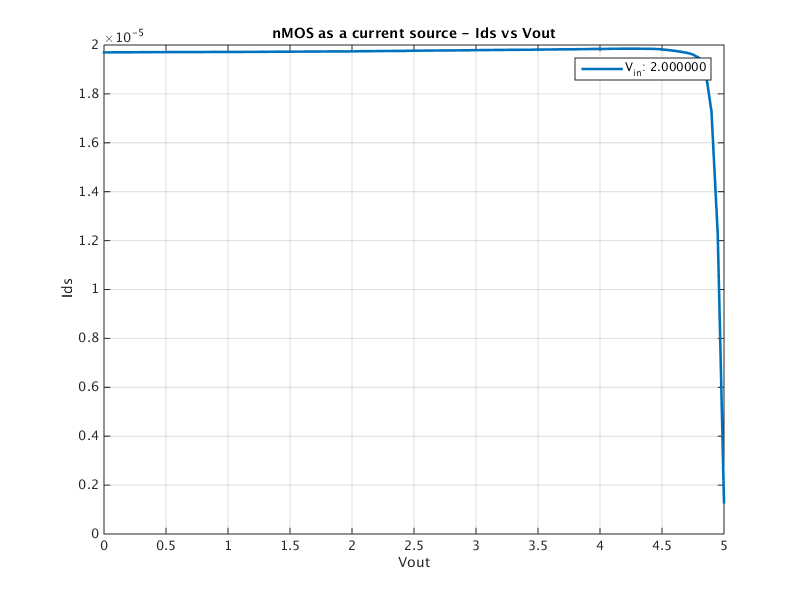
\includegraphics[width=\textwidth]{img/task4_nmos_as_a_current_source}}
  \caption{nMOS transistor as current source.}
  \label{fig:task4_plot}	
\end{figure}

Single stage amplifier.
\\
1. First we maually find the new $V_{n\_bias}$ for the first nmos transistor at 20 uA.\\
Uses the same nmos transistor as we did in the lab 1. (port 6(G),7(S) and 8(D))\\
2. Then we use the voltage that we found in the first task and use it in the next task, whis is applying one more nmos transistor. Here we
use the ports 9 (S), 10 (G) and 12 (D). (Reference to picture of setup)



%//////////////////////////////////////Task5///////////////////////////////////////////////////////////////////////
\section{Task 5}
We now want to determine a good DC voltage for the input for the amplifier. Since our goal is to have an output voltage 
verry close to $Vdd/2$, we need to find good bias voltages for $V_{n_bias1}$ and $V_{in}$. We found this volage to be $16 V$, 
in order to ensure that all transistors are operating. For the bias voltages we used the same relationships to $Vdd$ as in the previos tasks.\\

\begin{enumerate}
\item \itab{$V_{p_bias1}$:} \tab{1.19 V}
\item \itab{$V_{p_bias2}$:} \tab{3.39 V}     
\item \itab{$V_{n_bias1}$:} \tab{12.99V} 
      \tab{Almost 100\%} 
\item \itab{SPEC 04:} \tab{Exposure time}
      \tab{As short as we can get}
\item \itab{SPEC 05:} \tab{Resolution} 
      \tab{As high as time lets us}    
\item \itab{SPEC 06:} \tab{Technology} 
      \tab{Cadence AMS 0.35 opto}
\item \itab{SPEC 07:} \tab{Voltage} 
      \tab{3.3V}
\end{enumerate}

\begin{figure}[htbp]
 \centering
  \fbox{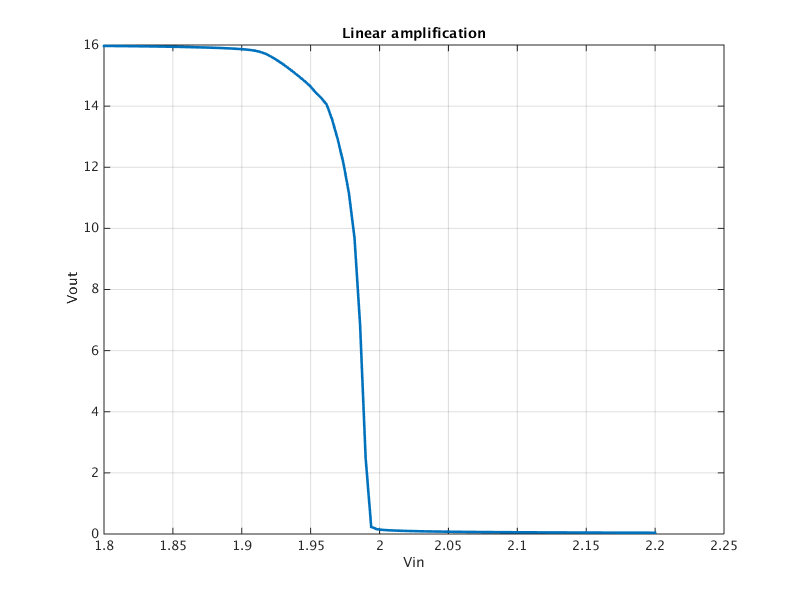
\includegraphics[width=\textwidth]{img/task5_vin_vs_vout}}
  \caption{Linear amplification.}
  \label{fig:lin-amp}	
\end{figure}

\begin{figure}[htbp]
 \centering
  \fbox{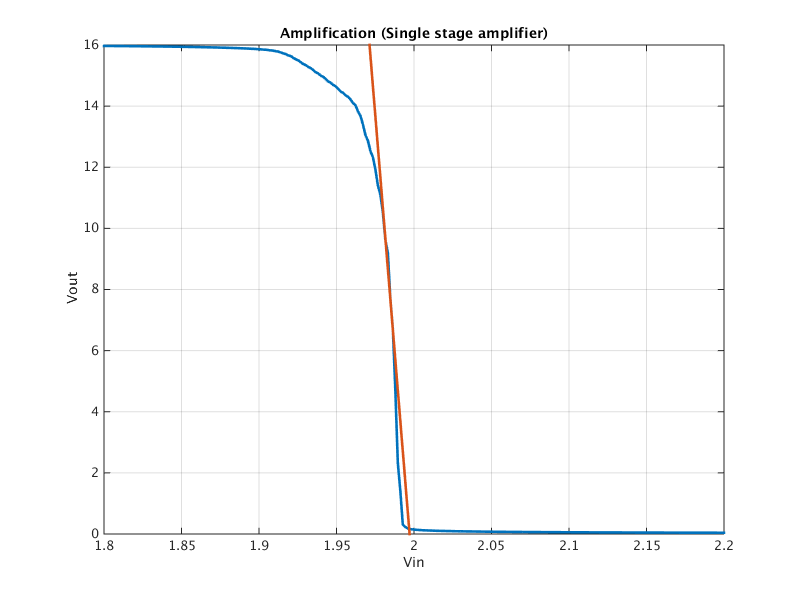
\includegraphics[width=\textwidth]{img/task5_single_stage_amplifier_tangent}}
  \caption{Linear amplification with tangent line.}
  \label{fig:lin-amp-tan}	
\end{figure}

%//////////////////////////////////////Task4///////////////////////////////////////////////////////////////////////
\section{Task 6}

%//////////////////////////////////////Task4///////////////////////////////////////////////////////////////////////
\section{Task 7}
Qestions to answer:\\
\\
If an external capacitance is used, what value? Exact value is needed.\\
Derive the shematics for the resistive division and include it in the plot.\\
Plot the -3dB frequency as well as the unity-gain frequency.\\
Plot the frequency responce of the gain bandwidth with measurement point for at least 20 frequencies, clearly covering the pass-band and cut-off regions.\\
How can we verify that the RC circuit is not dominating the cut-off?\\
Dokumenter alle stegene i denne oppgaven veldig detaljert.\\

\begin{figure}[htbp]
 \centering
  \fbox{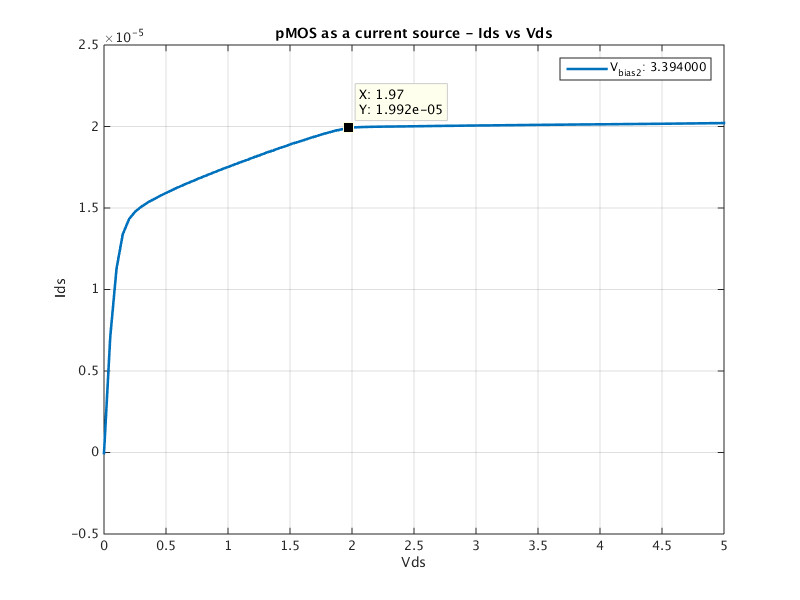
\includegraphics[width=\textwidth]{img/task2_pmos_as_a_current_source.png}}
  \caption{pFET and cascode pFET as a current cource.}
  \label{fig:pfet-cascode-pfet}	
\end{figure}

\end{document}
